
\section{The Small-World Model}

It should be clarified that real networks are not random. Their formation and development are dictated by a combination of many different processes and influences. These influencing conditions include natural limitations and processes, human considerations such as optimal performance and robustness, economic considerations, natural selection and many others. Controversies still exist regarding the measure to which random models represent real-world networks. However, in this chapter we will focus on random network models and attempt to show if their properties may still be used to study properties of real-world networks. \s

% [cite]
\noindent Many real-world networks have many properties that cannot be explained by the ER model. One such property is the high clustering observed in many real-world networks. This led Watts and Strogatz to develop an alternative model, called the “small-world” model. Their idea was to begin with an ordered lattice, such as the \emph{k-}ring (a ring where each site is connected to its $2k$ nearest neighbors - k from each side) or the two-dimensional lattice (see Figure \ref{fig:fig1}). For each site, each of the links emanating from it is removed with probability $\varphi$ and is rewired to a randomly selected site in the network. A variant of this process is to add links rather than rewire, which simplifies the analysis without considerably affecting the results. The obtained network has the desirable properties of both an ordered lattice (large clustering) and a random network (small world), as we will discuss below.

\begin{figure}[h]
    \centering
    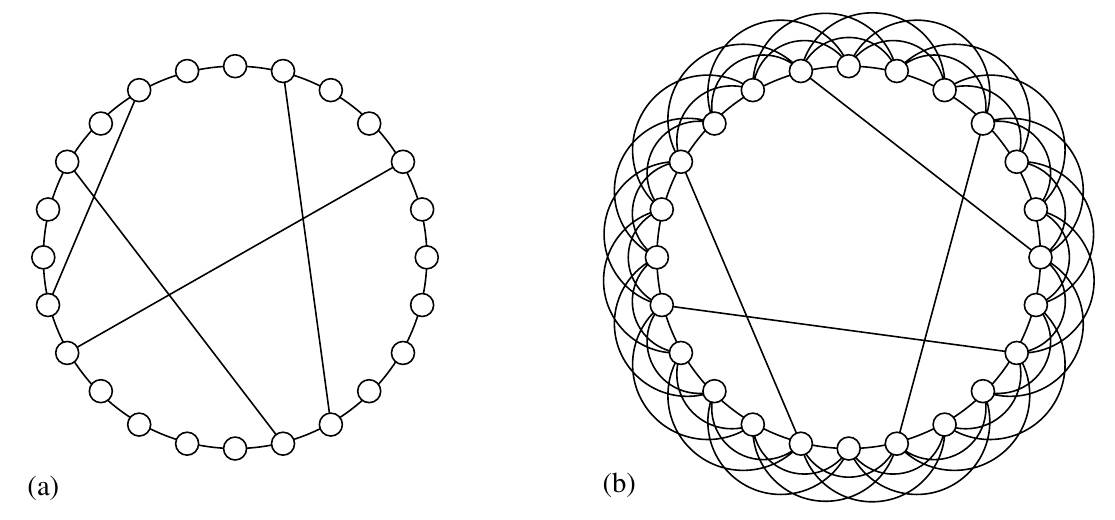
\includegraphics[width=0.9\textwidth]{figures/7olKNVY.png}
    \caption{Small-world networks with an underlying ring structure. (a) A small-world network formed by adding shortcuts to a simple ring (with $k = 1$). (b) A small-world network formed by adding shortcuts to a ring with $k = 3$.}
    \label{fig:fig1}
\end{figure}

\subsection{Clustering in a small-world network}

\nd The simplest way to treat clustering analytically in a small-world network is to use the link addition, rather than the rewiring model. In the limit of large network size, $N \to \infty$, and for a fixed fraction of shortcuts $\phi$, it is clear that the probability of forming triangle vanishes as we approach $1/N$, so the contribution of the shortcuts to the clustering is negligible. Therefore, the clustering of a small-world network is determined by its underlying ordered lattice. For example, consider a ring where each node is connected to its $k$ closest neighbors from each side. A node's number of neighbors is therefore $2k$, and thus it has $2k(2k - 1)/2 = k(2k - 1)$ pairs of neighbors. Consider a node, $i$. All of the $k$ nearest nodes on $i$'s left are connected to each other, and the same is true for the nodes on $i$'s right. This amounts to $2k(k - 1)/2 = k(k - 1)$ pairs. Now consider a node located $d$ places to the left of $k$. It is also connected to its $k$ nearest neighbors from each side. Therefore, it will be connected to $k - d$ neighbors on $i$'s right side. The total number of connected neighbor pairs is

\begin{equation}
    k(k-1) + \sum_{d=1}^k (k-d) = k(k-1) + \frac{k(k-1)}{2} = \frac{{3}{2}} k (k-1)
\end{equation}

\nd and the clustering coefficient is:

\begin{equation}
    C = \frac{\frac{3}{2}k(k-1)}{k(2k-1)} =\frac{3 (k-1)}{2(2k-1)}
\end{equation}

\nd For every $k > 1$, this results in a constant larger than $0$, indicating that the clustering of a small-world network does not vanish for large networks. For large values of $k$, the clustering coefficient approaches $3/4$, that is, the clustering is very high. Note that for a regular two-dimensional grid, the  clustering by definition is zero, since no triangles exist. However, it is clear that the grid has a neighborhood structure.

\subsection{Distances in a small-world network}

The second important property of small-world networks is their small diameter, i.e., the small distance between nodes in the network. The distance in the underlying lattice behaves as the linear length of the lattice, L. Since $N \sim L^d$  where $d$ is the lattice dimension, it follows that the distance between nodes behaves as:

\begin{equation}
    l \sim L \sim N^{1/d}
\end{equation}

\nd Therefore, the underlying lattice has a finite dimension, and the distances on it behave as a power law of the number of nodes, i.e., the distance between nodes is large. However, when adding even a small fraction of shortcuts to the network, this behavior changes dramatically. \s

\nd Let's try to deduce the behavior of the average distance between nodes. Consider a small-world network, with dimension d and connecting distance $k$ (i.e., every node is connected to any other node whose distance from it in every linear dimension is at most $k$). Now, consider the nodes reachable from a source node with at most $r$ steps. When $r$ is small, these are just the \emph{r-th} nearest neighbors of the source in the underlying lattice. We term the set of these neighbors a “patch”. the radius of which is $kr$ , and the number of nodes it contains is approximately $n(r) = (2kr)d$. \s

\nd We now want to find the distance r for which such a patch will contain about one shortcut. This will allow us to consider this patch as if it was a single node in a randomly connected network. Assume that the probability for a single node to have a shortcut is $\Phi$. To find the length for which approximately one shortcut is encountered, we need to solve for $r$ the following equation: $(2kr)^d \Phi = 1$. The correlation length $\xi$ defined as the distance (or linear size of a patch) for which a shortcut will be encountered with high probability is therefore,

\begin{equation}
    \xi = \frac{1}{k \Phi^{1/d}}
\end{equation}

\nd Note that we have omitted the factor 2, since we are interested in the order of magnitude. Let us denote by $V(r)$ the total number of nodes reachable from a node by at most $r$ steps, and by $a(r)$, the number of nodes added to a patch in the \emph{r-th} step. That is, $a(r) = n(r) - n(r-1)$. Thus,

\begin{equation}
    a(r) \sim \frac{\text{d} n(r)}{\text{d} r} = 2kd(2kr)^{d-1}
\end{equation}

\nd When a shortcut is encountered at the r step from a node, it leads to a new patch \footnote{It may actually lead to an already encountered patch, and two patches may also merge after some steps, but this occurs with negligible probability when $N \to \infty$ until most of the network is reachable}. This new patch occurs after $r'$ steps, and therefore the number of nodes reachable from its origin is $V (r - r')$. Thus, we obtain the recursive relation

\begin{equation} \label{eq:recursion}
    V(r) = \sum_{r'=0}^r a(r') [1 + \xi^{-d}V(r-r')]
\end{equation}

\nd where the first term stands for the size of the original patch, and the second term is derived from the probability of hitting a shortcut, which is approximately $\xi -d $ for every new node encountered. To simplify the solution of \ref{eq:recursion}, it can be approximated by a differential equation. The sum can be approximated by an integral, and then the equation can be differentiated with respect to $r$ . For simplicity, we will concentrate here on the solution for the one-dimensional case, with $k = 1$, where $a(r) = 2$. Thus, one obtains

\begin{equation}
    \frac{\text{d} V(r)}{\text{d} r} = 2 [1 + V(r)/\xi]
\end{equation}

\nd the solution of which is:

\begin{equation} \label{eq:V(r)}
    V(r) = \xi \left(e^{2r/\xi} -1\right)
\end{equation}

\nd For $r \ll \xi$, the exponent can be expanded in a power series, and one obtains $V(r) \sim 2r = n(r)$, as expected, since usually no shortcut is encountered. For $r \ gg \xi$, $V(r)$. An approximation for the average distance between nodes can be obtained by equating $V(r)$ from \ref*{eq:V(r)} to the total number of nodes, $V(r) = N$. This results in

\begin{equation} \label{eq:average distance}
    r \sim \frac{\xi}{2} \ln \frac{N}{\xi}
\end{equation}

\nd As apparent from \ref{eq:average distance}, the average distance in a small-world network behaves as the distance in a random graph with patches of size $\xi$ behaving as the nodes of the random graph.
